\documentclass[a4paper,11pt]{article}
\usepackage[T1]{fontenc}
\usepackage[utf8]{inputenc}
\usepackage[top=1in, bottom=1in, left=0.75in, right=0.5in]{geometry}
\usepackage{amsmath}
\usepackage{graphicx}

\title{Timing and Profiling Code: A Group 09 Report}
\author{
  Deepali Adlakha\\
  \texttt{11D170020}\\
  \texttt{dadlakha0111@gmail.com}
  \and
  K. Kartik Pranav\\
  \texttt{110050062}\\
  \texttt{kartikpranav.k@gmail.com}
  \and
  Vibhor Kanojia\\
  \texttt{110050036}\\
  \texttt{versatilevibhor@gmail.com}
}

\date{2nd March, 2013}

\begin{document}

\maketitle

\section{Introduction}
The following is a report as part of Lab 7 of CS 296. It attempts to analyze the time results obtained in Lab 5, and infer some interesting results from the timing experiments and plots. Later, the profiling of the base code is done, and optimization flags are used to try and find out where the code can be optimized.

\section{The Timing Part}
In Lab 5, we have used gettimeofday to obtain the time taken in various measurements. The iteration values were from 1 to 100, and each one was rerun 100 times. Using the data obtained, we plotted 6 pairs of graphs.\\\\
In each pair, the average times (step, collision, velocity update and position update) have increased when the system was heavily loaded with processes, so the times are higher overall. The changes in the two cases are discussed for each plot:

\subsection*{Plot 01}

\begin{center}
  \includegraphics[scale=0.35]{doc/oldone/g09_plot01.eps}
  \includegraphics[scale=0.35]{doc/newone/g09_plot01.eps}
\\  Loaded~~~~~~~~~~~~~~~~~~~~~~~ Unloaded  
\end{center}

In the first plot, the processor does scheduling and prioritizes the processes on the basis of the time they are going to take. So, when there are a larger number of iterations to do, it increases its speed, so the step time decreases with iterations.\\
The loop time is the cumulative sum of step times. Since the step times are decreasing, the loop time increases at a slower rate.

\subsection*{Plot 02}

\begin{center}
  \includegraphics[scale=0.35]{doc/oldone/g09_plot02.eps}
  \includegraphics[scale=0.35]{doc/newone/g09_plot02.eps}
\\  Loaded~~~~~~~~~~~~~~~~~~~~~~~ Unloaded  
\end{center}

In the second plot, we see that the step time is decreasing, as inferred from Plot 1. Thus, the collision time, velocity update time and position update time are all decreasing, with step time being the maximum out of the four.\\
The collision time is less than the other two because it is caluclated in the $Collide$ function, which finds the time taken in the  $PreSolve$ and $PostSolve$ functions called repeatedly under it.\\
Velocity update and position update are calculated in the $Solve$ function, which uses simple momentum conservation formulae and at each step, calculates whether there will be a collision or not.

\subsection*{Plot 03}

\begin{center}
  \includegraphics[scale=0.35]{doc/oldone/g09_plot03.eps}
  \includegraphics[scale=0.35]{doc/newone/g09_plot03.eps}
\\  Loaded~~~~~~~~~~~~~~~~~~~~~~~ Unloaded  
\end{center}

In the third plot, the time values are very close for all the reruns because the iteration value is the same in the graph.\\
The order of the four times is similar to that obtained from Plot 2.

\subsection*{Plot 04}

\begin{center}
  \includegraphics[scale=0.35]{doc/oldone/g09_plot04.eps}
  \includegraphics[scale=0.35]{doc/newone/g09_plot04.eps}
\\  Loaded~~~~~~~~~~~~~~~~~~~~~~~ Unloaded  
\end{center}

The fourth plot is similar to the thrid, in that it is being plotted over the same iteration value, so the times are nearly the same.

\subsection*{Plot 05}

\begin{center}
  \includegraphics[scale=0.35]{doc/oldone/g09_plot05.eps}
  \includegraphics[scale=0.35]{doc/newone/g09_plot05.eps}
\\  Loaded~~~~~~~~~~~~~~~~~~~~~~~ Unloaded  
\end{center}

In the fifth plot, the step time decreases over the iteration value, due to the same reason inferred in Plot 1, the processor's scheduling.\\
Also, the standard deviation decreases over the iteration value because the number of sample points in increasing. This means that the mean will be closer to the ovtained values, and so the deviation decreases.

\subsection*{Plot 06}

\begin{center}
  \includegraphics[scale=0.35]{doc/oldone/g09_plot06.eps}
  \includegraphics[scale=0.35]{doc/newone/g09_plot06.eps}
\\  Loaded~~~~~~~~~~~~~~~~~~~~~~~ Unloaded  
\end{center}

In the sixth plot, we compare the loaded and unloaded plots. In the latter, the peak is obtained at a step time of around 0.65, whereas in the former, the peak is at around 0.8. This is because the process is taking more time in the case of a loaded system.

\section{The Profiling Part}
The profiling of the CS 296 base code is done here with GProf. We compare two versions of the code, the $Release$ and the $Debug$ versions. The former uses the optimization flag $-O3$ for near-maximum optimization, whereas the latter uses no such flags, executing the original version of the code, as is.

\subsection*{Inlining Functions}
Comparing the two flat profiles generated by GProf, we see that in the optimized case, there are relatively very few function calls. This is because the $-O3$ flag includes, among others, the -finline-function optimization, which makes sure that all functions used have been expanded inline. Meaning that in every place that a function is called, the body of the function is inserted to reduce function calls.\\\\
Due to this, some functions have been expanded inline, and not called at all, such as $b2Vec2()$, with approx. 67M calls, and the overloaded - and * operators, with around 2M calls each.

\subsection*{Unrolling Loops}
With the option -funroll-loops, most loops are unrolled completely, expanding the code. This may or may not make the code faster, but it is useful in most cases to increase a program's speed by reducing instructions that control the loop.\\
Loops can be re-written instead as a repeated sequence of similar independent statements eliminating this overhead. $[Wikipedia]$

\subsection*{Reusing Computed Values}
-fpredictive-commoning performs predictive commoning optimization, which means the reusing of computations performed in previous iterations of loops.\\
This can save a lot of time in programs such as a Box2D simulation, where an iteration of a loop may be highly dependent on a previous iteration.

\subsection*{Reordering Blocks and Functions}
There are two optimizations, -freorder-blocks and -freorder-functions, that improve code locality. The first reorders the basic blocks in the compiled function, whereas in the latter, the reordering of functions is done by the linker.

\subsection*{Aligning Loops, Functions and Labels}
The options -falign-loops, -falign-functions and -falign-labels align the respective object to the next power-of-2 boundary. The expectation is that the function (loop, etc.) would be called multiple times, which makes up for execution of any dummy operations.\\\\
On comparing the two flat profiles, we see that the function $SolveVelocityConstraint()$ from $b2ContactSolver$ could be optimized, as it is the function that takes the maximum amount of time during execution.
Also, $b2ContactListener$ has a couple of functions that have hundreds of thousands of calls (not removed even when inlining of functions is done), so these could improved upon, to improve running time.

\section*{The Call Graph}
The profiling of code done by GProf generates an analysis file, one part of which is the flat profile, used above.\\
The other part is the $call~graph$, which shows how much time was spent in every function (and functions called inside each). We can find functions that called others which used a large amount of time, even if the original function did not use much itself.\\\\
Drawing the call graph as an image using the gprof2dot Python script, we can view the same thing visually.\\\\

In this case, here is call graph for the Debug version of the CS 296 base code:\\

\begin{center}
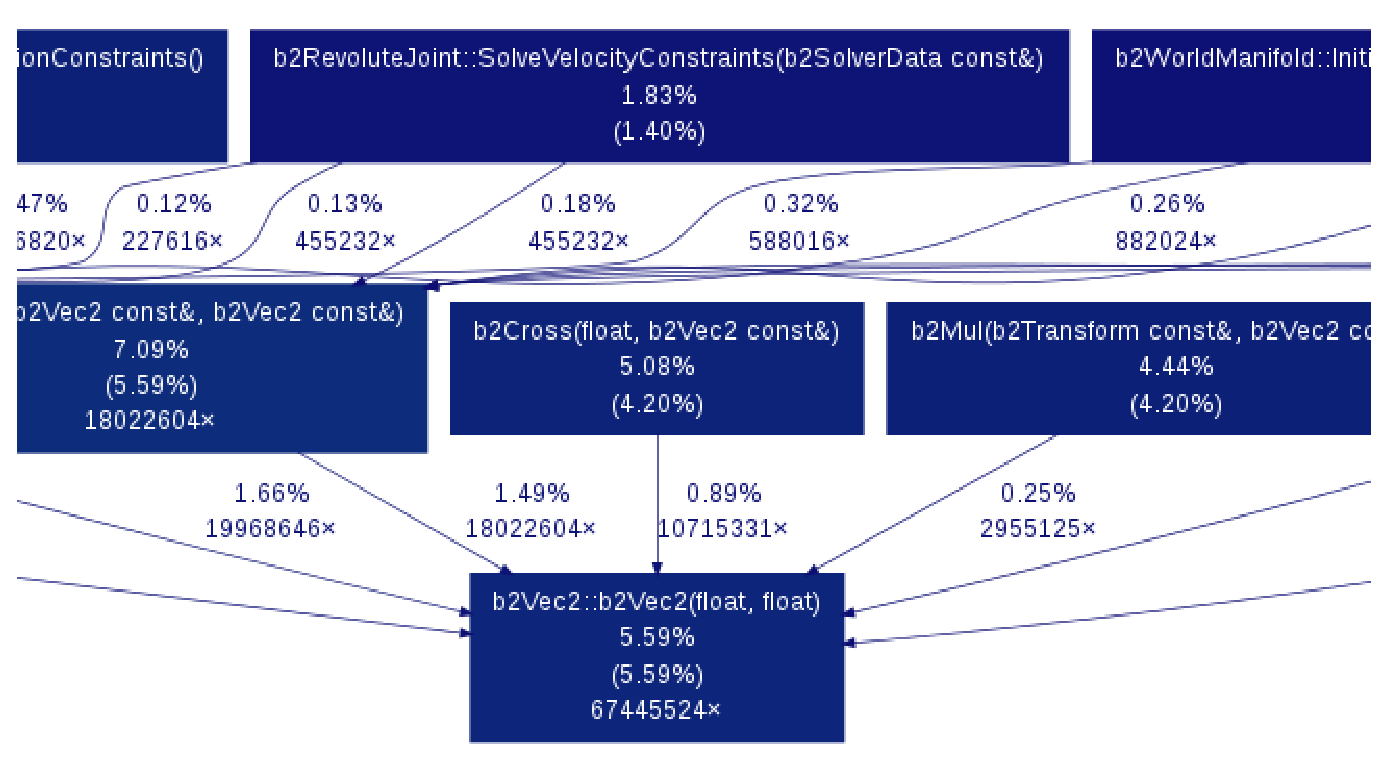
\includegraphics[scale=0.6]{doc/output.eps}
\end{center}

Here, many functions contain the function $b2Vec2$, and this results in many calls (around 67M). However, the call graph of the optimized version of the code generates a straight line of function blocks. This is due to function inlining, so that no function has to call others inside. So, we can see from the call graph that function inlining is a very efficient way of reducing running time.

\section{Conclusion}
In this assignment, we got to learn how Box2D functions work. We analyzed the various plots produced in Lab5. We also found out about the various optimization options, and what they can do to improve the running time.
\end{document}
